\block{}{
 	{ \fontsize{40}{40}\selectfont 
	
	\vspace{-1em}
	\section{Extraction des caractéristiques}
	\vspace{-0.5em}
	La \textbf{GLCM} (\textit{Gray-Level Co-occurrence Matrix}) ou matrice de co-occurrences a été proposée par Haralick et al. \cite{ref_03}. Elle permet d'analyser les textures en calculant les répartitions des différents des niveaux de gris dans l'image en se basant sur les positions relatives des pixels.\vspace{0.5em}  

	Il est possible de l'utiliser directement et appliquer la \textit{réduction de dimensionnalité} ou bien extraire différentes caractéristiques comme le contraste, l'énergie, l'homogénéité, etc.
	
    \begin{center}
        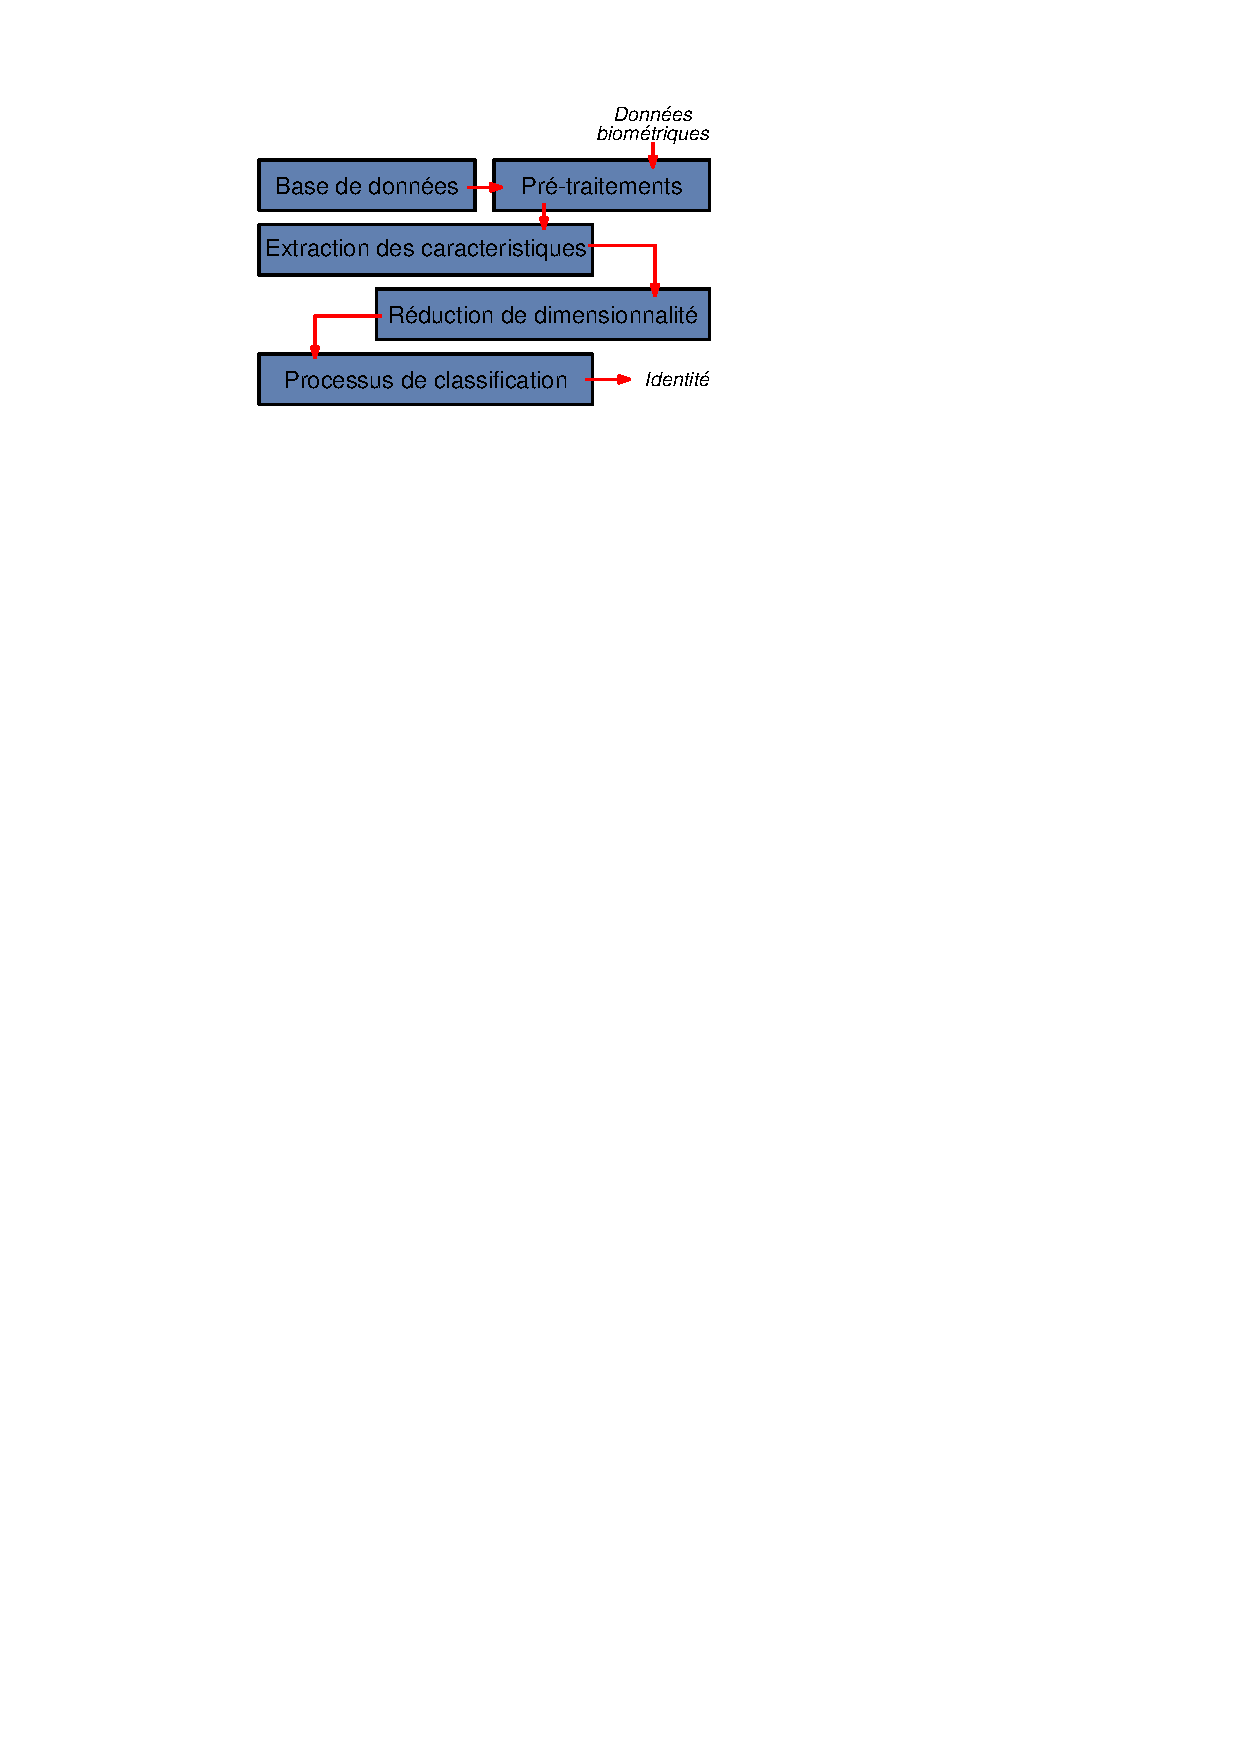
\includegraphics[width=0.8\linewidth]{schema.pdf}
        \vspace{0.3em}
        \captionof{figure}{\label{fig_01}Les différents blocs du système biométrique.}
    \end{center}
	
	\vspace{-1em}
	\section{Réduction de la dimensionnalité}
	\vspace{-0.5em}
	C'est un processus qui consiste à réduire considérablement la taille du vecteur de caractéristiques dans le but de faciliter le processus d'apprentissage.\vspace{0.5em}  
	
	La méthode utilisée est la \textbf{PCA} (\textit{Principal Component Analysi}s) ou l'analyse en composantes principales. Durant le processus de projection et transformation, seule l'information utile est conservée.
	
	\vspace{-1em}
	\section{Processus de classification}
	\vspace{-0.5em}
	Une technique d'apprentissage machine \textit{supervisée} a été utilisée. C'est le $k$-\textbf{NN} ($k$-\textit{Nearest Neighbors}) ou la méthode des $k$ plus proches voisins. \vspace{0.5em}  
	
	Le $k$-\textbf{NN} consiste à trouver les $k$ échantillons à partir de la base de données de référence et qui se rapproche le plus de l'échantillon d'entrée. Le critère utilisé est la distance de \textit{Manhattan}. C'est sur la base d'un vote de majorité sur les $k$ échantillons que l'identité est déterminée.
	
	}
}